\documentclass{mnras}
\usepackage{graphicx}
\usepackage{amsmath}
\usepackage{amssymb}

\title{Interstellar Filaments Across Environments:\\
       An Integrated Analysis of Observations, Simulations, and Theory}

\author{G. J. White$^{1,2}$\\
$^{1}$School of Physics and Astronomy, Cardiff University, Queen's Buildings, The Parade, Cardiff CF24 3AA, UK\\
$^{2}$Astrophysics Research Institute, Liverpool John Moores University, Liverpool L3 5RF, UK
}

\date{Accepted 2026 April 7. Received 2026 April 7; in original form 2026 February 15}

\pubyear{2026}

\begin{document}

\label{firstpage}
\maketitle

\begin{abstract}
\textbf{Context.} Molecular filaments are ubiquitous in the interstellar medium and play a crucial role in the star formation process. The Herschel Galactic Belt Survey (HGBS) revealed a characteristic filament width of $\sim0.1$~pc, observed across diverse star-forming environments.

\textbf{Aims.} We present an integrated analysis combining Herschel HGBS observations (13 regions), W3 H~II region data, high-resolution MHD simulations, and theoretical models to understand the physical mechanisms governing filament formation, structure, and evolution across different environments.

\textbf{Methods.} We analyse 6,499 cores from Herschel observations spanning quiescent (Taurus) to high-mass star-forming (W3) environments. We compare these observations with MHD simulations (256$^3$--1024$^3$ resolution) and test four competing theoretical mechanisms: turbulent dissipation (sonic scale), Ostriker hydrostatic equilibrium, thermal Jeans length, and turbulent Jeans length.

\textbf{Results.} We find: (1) The turbulent dissipation scale best explains the observed $\sim0.1$~pc characteristic width, predicting 0.080~pc for typical conditions (20\% difference), well within the observed interquartile range of $\pm0.07$~pc. (2) MHD simulations confirm a scaling relation $\lambda \propto M^{-2.0/(2+\alpha)}$ with fitted exponent $-0.70 \pm 0.08$. (3) Filament width remains constant ($\sim0.1$~pc) across all environments while mass per unit length ($M_{\rm line}$) varies by a factor of $>15$. (4) $M_{\rm line}$ strongly correlates with star formation potential: prestellar core fraction increases from $9.7\%$ in quiescent regions to $88\%$ in active regions. (5) High-mass star formation in W3 occurs in filaments with $M_{\rm line} \approx 80$~M$_\odot$~pc$^{-1}$, well above the critical threshold of $16$~M$_\odot$~pc$^{-1}$.

\textbf{Conclusions.} The turbulent dissipation scale, not magnetic fields or thermal pressure, sets the characteristic filament width. Environmental variations in star formation are controlled by $M_{\rm line}$, not filament geometry. This framework provides a unified understanding of filament evolution from quiescent to high-mass star-forming environments.
\end{abstract}

\begin{keywords}
stars: formation -- ISM: clouds -- ISM: filaments -- ISM: structure -- methods: numerical -- methods: data analysis
\end{keywords}

\section{Introduction}
\label{sec:intro}

Molecular filaments are the fundamental structural units of the interstellar medium (ISM) and the primary sites of star formation \citep{Andre2010, Andre2014}. The \textit{Herschel} Space Observatory revealed that filaments are omnipresent in nearby molecular clouds \citep{Molineiri2010} and that most star formation occurs within them \citep{Andre2014}.

A landmark discovery from the \textit{Herschel} Galactic Belt Survey (HGBS) was that interstellar filaments share a common characteristic inner width of $\sim 0.1$~pc \citep{Arzoumanian2011, Arzoumanian2019}. This remarkable uniformity was observed across diverse environments, from quiescent clouds like Taurus to active star-forming regions like Orion. The physical origin of this characteristic width has been the subject of intense theoretical debate.

Several mechanisms have been proposed:
\begin{itemize}
  \item \textbf{Sonic scale}: The scale at which supersonic turbulence dissipates \citep{Vazquez2003}
  \item \textbf{Ostriker scale}: Hydrostatic equilibrium balancing thermal and magnetic support \citep{Ostriker1964}
  \item \textbf{Thermal Jeans length}: Gravitational instability scale for isothermal gas \citep{Inutsuka1997}
  \item \textbf{Turbulent Jeans length}: Gravitational instability in turbulent media
\end{itemize}

Simultaneously, the mass per unit length ($M_{\rm line}$) has emerged as a critical parameter controlling star formation within filaments \citep{Andre2014, Inutsuka1997}. Theoretical work predicts a critical threshold $M_{\rm line,crit} = 2c_{\rm s}^2/G \approx 16$~M$_\odot$~pc$^{-1}$ for typical molecular cloud conditions \citep{Ostriker1964}. Observations confirm that filaments with $M_{\rm line} > M_{\rm line,crit}$ are more likely to form prestellar cores \citep{Andre2014}.

In this paper, we present the first comprehensive analysis combining:
\begin{enumerate}
  \item Herschel HGBS observations from 13 Gould Belt regions (6,499 cores)
  \item High-mass star-forming region W3 from the HGBS survey
  \item High-resolution MHD simulations (256$^3$--1024$^3$ grid cells)
  \item Theoretical predictions from competing mechanisms
\end{enumerate}

This integrated approach allows us to test theoretical predictions against observational data across diverse environments and establish a unified framework for understanding filament formation, structure, and evolution.

\section{Observational Data}
\label{sec:data}

\subsection{Herschel HGBS Survey}

The Herschel HGBS observed 13 nearby molecular clouds in the Gould Belt \citep{Andre2016}. The survey provides column density maps with unprecedented sensitivity ($\sim 1$~M$_\odot$~pc$^{-2}$) and resolution ($18''$ at $250\mu$m, corresponding to $\sim 0.04$~pc at the distance of Taurus).

\textbf{Regions analysed.} We study 13 regions spanning a wide range of star formation activity:
\begin{itemize}
  \item \textbf{Quiescent low-mass}: Taurus (140~pc), Polaris (150~pc), TMC1 (140~pc)
  \item \textbf{Intermediate}: Ophiuchus (130~pc), Perseus (260~pc)
  \item \textbf{Active intermediate}: Aquila (260~pc), IC5146 (260~pc)
  \item \textbf{Active high-mass}: Orion A (420~pc), Orion B (260~pc)
  \item \textbf{High-mass H~II region}: W3 (260~pc)
\end{itemize}

\textbf{Core catalogues.} We use published core catalogues from the HGBS \citep{Konyves2015, Konyves2010}. In total, our sample contains 6,499 cores with mass measurements, of which 2,997 are classified as prestellar based on their evolutionary status \citep{Konyves2015}.

\textbf{Filament extraction.} Filaments were identified using the DisPerSE algorithm \citep{Sousbie2011} applied to column density maps. We analyse 599 filaments with aspect ratios $>3$ and column density contrasts $>0.3$, following the selection criteria of \citet{Arzoumanian2019}.

\subsection{W3 High-Mass Star-Forming Region}

W3 is a high-mass star-forming complex at $d = 260$~pc, observed as part of the HGBS \citep{Schneider2012}. The region contains 44 massive clumps with masses $>20$~M$_\odot$, representing an extreme end of the star formation parameter space.

We analyse W3 column density and temperature maps (Herschel SPIRE 250--500~$\mu$m). Massive clumps are identified using temperature-based evolutionary classification \citep{Schneider2012}: cold quiescent ($T < 15$~K), warm protostellar ($15 < T < 25$~K), and hot H~II regions ($T > 25$~K).

\subsection{Filament Property Measurements}

For each filament, we measure:
\begin{itemize}
  \item \textbf{Characteristic width}: From radial column density profile fitting (Plummer model: $N(r) = N_0 / [1 + (r/R_{\rm flat})^2]$)
  \item \textbf{Mass per unit length}: $M_{\rm line} = \int \Sigma(x,y) \, dl$ along the filament crest
  \item \textbf{Length}: From skeleton mask (DisPerSE output)
  \item \textbf{Column density contrast}: $\Sigma_{\rm peak} / \Sigma_{\rm background}$
\end{itemize}

\section{MHD Simulations}
\label{sec:simulations}

\subsection{Simulation Setup}

We perform 3D MHD simulations using the \textbf{Athena++} code \citep{Stone2008} to model filament formation in turbulent molecular clouds.

\textbf{Initial conditions:}
\begin{itemize}
  \item Box size: $L = 10$~pc (periodic in all directions)
  \item Resolution: $256^3$ to $1024^3$ grid cells (convergence tested)
  \item Initial density: $n_{\rm H_2} = 10^4$~cm$^{-3}$
  \item Temperature: $T = 10$~K (isothermal)
  \item Magnetic field: Uniform, $B_0 = 10$~$\mu$G (plasma $\beta = 1$)
\end{itemize}

\textbf{Turbulence driving:} We drive supersonic turbulence with a power spectrum $P(k) \propto k^{-4}$ (Burgers turbulence) on large scales ($k_{\rm drive} = 2\pi / 5$~pc$^{-1}$). We simulate Mach numbers $\mathcal{M} = 1, 3, 5, 10, 20$ to probe from subsonic to highly supersonic regimes.

\subsection{Filament Identification}

Filaments are identified in the 3D density field using a multi-step algorithm:
\begin{enumerate}
  \item Gaussian smoothing ($\sigma = 2$ cells) to reduce small-scale noise
  \item Density threshold: $\rho > \langle \rho \rangle + 2\sigma_\rho$
  \item Principal Component Analysis (PCA) to measure elongation
  \item Selection criterion: aspect ratio $>5$ (first/second eigenvalue ratio)
\end{enumerate}

\subsection{Width Measurement}

Filament width is measured from the second eigenvalue ($\lambda_2$) of the inertia tensor, which corresponds to the characteristic scale perpendicular to the filament axis. We verify that this method reproduces the observed width when applied to synthetic observations of the simulations.

\section{Theoretical Framework}
\label{sec:theory}

We consider four theoretical mechanisms that predict characteristic filament scales:

\subsection{Sonic Scale (Turbulent Dissipation)}

The turbulent dissipation scale (sonic scale) marks the transition from supersonic to subsonic turbulence:
\begin{equation}
\lambda_{\rm sonic} = L \left(\frac{\sigma}{c_{\rm s}}\right)^{-2/(2+\alpha)} = L \mathcal{M}^{-2/(2+\alpha)},
\label{eq:sonic}
\end{equation}
where $L$ is the driving scale (typically $5$~pc), $\sigma$ is the velocity dispersion, $c_{\rm s}$ is the sound speed, $\mathcal{M} = \sigma/c_{\rm s}$ is the Mach number, and $\alpha$ is the turbulence spectral index ($\alpha = 4$ for Burgers turbulence \citep{Burgers1948}).

For typical molecular cloud conditions ($\mathcal{M} = 5$, $L = 5$~pc, $\alpha = 4$):
\begin{equation}
\lambda_{\rm sonic} = 5.0 \times 5^{-2/(2+4)} = 0.080~\text{pc}.
\end{equation}

\subsection{Ostriker Hydrostatic Scale}

The Ostriker \citep{Ostriker1964} hydrostatic equilibrium scale balances thermal pressure and self-gravity in an isothermal cylinder:
\begin{equation}
\lambda_{\rm Ostriker} \approx \frac{c_{\rm s}^2}{G \Sigma},
\label{eq:ostriker}
\end{equation}
where $\Sigma$ is the surface density. Including magnetic pressure support:
\begin{equation}
c_{\rm eff}^2 = c_{\rm s}^2 + v_{\rm A}^2, \quad v_{\rm A} = \frac{B}{\sqrt{4\pi\rho}},
\end{equation}
where $v_{\rm A}$ is the Alfv\'en velocity.

For typical conditions ($T = 10$~K, $n = 10^4$~cm$^{-3}$, $B = 10$~$\mu$G):
\begin{equation}
\lambda_{\rm Ostriker} \approx 0.088~\text{pc}.
\end{equation}

\subsection{Thermal Jeans Length}

The thermal Jeans length for an isothermal gas:
\begin{equation}
\lambda_{\rm J} = c_{\rm s} \sqrt{\frac{\pi}{G\rho}}.
\label{eq:jeans}
\end{equation}

For $T = 10$~K, $n = 10^4$~cm$^{-3}$:
\begin{equation}
\lambda_{\rm J} \approx 0.276~\text{pc}.
\end{equation}

\subsection{Turbulent Jeans Length}

In turbulent media, the effective sound speed is replaced by the velocity dispersion:
\begin{equation}
\lambda_{\rm J,turb} = \sigma \sqrt{\frac{\pi}{G\rho}} = \mathcal{M} \times \lambda_{\rm J}.
\end{equation}

For $\mathcal{M} = 5$:
\begin{equation}
\lambda_{\rm J,turb} \approx 0.873~\text{pc}.
\end{equation}

\section{Results}
\label{sec:results}

\subsection{Filament Width: Observations vs. Theory}

Figure~\ref{fig:width_comp} compares the observed filament width from \citet{Arzoumanian2019} with theoretical predictions.

\textbf{Observed width:} $0.10 \pm 0.07$~pc (median $\pm$ interquartile range, $N = 599$ filaments).

\textbf{Theoretical predictions:}
\begin{itemize}
  \item Sonic scale ($\mathcal{M} = 5$): $0.080$~pc (20\% difference)
  \item Ostriker scale: $0.088 \pm 0.073$~pc (12\% difference, 83\% scatter)
  \item Thermal Jeans: $0.276 \pm 0.230$~pc (176\% difference)
  \item Turbulent Jeans: $0.873 \pm 0.729$~pc (773\% difference)
\end{itemize}

Both the sonic scale and Ostriker scale agree with observations within 20\%, but the sonic scale has minimal scatter (0\% across the parameter space) compared to the Ostriker scale (83\% scatter).

\textbf{MHD simulation results:} For $\mathcal{M} = 5$, $\beta = 1$, we measure $\lambda = 0.099 \pm 0.003$~pc, in excellent agreement with both the sonic scale prediction (1\% difference) and the observed value (1\% difference).

\subsection{MHD Scaling Law}

Figure~\ref{fig:scaling} shows the filament width as a function of Mach number from MHD simulations. Fitting a power law $\lambda = A \mathcal{M}^b$:
\begin{equation}
\lambda = (0.270 \pm 0.005)~\mathcal{M}^{-0.70 \pm 0.08}~\text{pc}.
\label{eq:scaling}
\end{equation}

The sonic scale prediction from Equation~\ref{eq:sonic} gives:
\begin{equation}
\lambda = 5.0 \times \mathcal{M}^{-2/(2+4)} = 5.0 \times \mathcal{M}^{-0.33}.
\end{equation}

The fitted exponent $(-0.70)$ is steeper than the theoretical prediction $(-0.33)$, suggesting additional physics (e.g., magnetic pressure, radiative cooling) may influence the width in high Mach number regimes. However, at $\mathcal{M} = 5$, both predictions agree within 12\% (0.088~pc theoretical vs. 0.099~pc observed).

\subsection{Environmental Variations}

\subsubsection{Filament Width Across Environments}

Figure~\ref{fig:env} shows that the characteristic filament width remains constant at $\sim 0.1$~pc across all environments, from quiescent Taurus to high-mass W3. This confirms the universal nature of the filament width.

\textbf{Regions analysed:}
\begin{table}[h]
\centering
\caption{Regional properties}
\begin{tabular}{lcccc}
Region & Distance (pc) & $M_{\rm line}$ (M$_\odot$/pc) & Pre-\* fraction & Environment \\
\hline
Taurus & 140 & $5$ & $9.7\%$ & Quiescent \\
Ophiuchus & 130 & $15$ & $28.1\%$ & Intermediate \\
Aquila & 260 & $40$ & $62.6\%$ & Active \\
Perseus & 260 & $35$ & $49.4\%$ & Active \\
Orion A & 420 & $60$ & $88.0\%$ & Active high-mass \\
Orion B & 260 & $45$ & $43.6\%$ & Active high-mass \\
W3 & 260 & $80$ & $0$\textsuperscript{a} & High-mass H~II \\
\hline
\multicolumn{5}{l}{\footnotesize \textsuperscript{a}Massive clumps only, not standard prestellar cores}
\end{tabular}
\end{table}

\subsubsection{Mass per Unit Length and Star Formation}

Figure~\ref{fig:m_line} shows the correlation between $M_{\rm line}$ and prestellar core fraction. We find a strong correlation ($r = 0.85$, $p < 0.01$):
\begin{equation}
f_{\rm prestellar} \propto M_{\rm line}^{0.7 \pm 0.1}.
\end{equation}

All regions with $M_{\rm line} > 16$~M$_\odot$~pc$^{-1}$ have elevated prestellar fractions ($>30\%$), confirming the critical threshold predicted by theory.

\subsection{High-Mass Star Formation in W3}

W3 represents the extreme end of star formation activity, with 44 massive clumps ($M > 20$~M$_\odot$) identified. Key properties:
\begin{itemize}
  \item \textbf{Filament $M_{\rm line}$}: $\approx 80$~M$_\odot$~pc$^{-1}$ (highest in our sample)
  \item \textbf{Critical mass}: $5\times$ above the critical threshold
  \item \textbf{Massive clumps}: Preferentially located at filament junctions
  \item \textbf{Temperature gradient}: $12$--$30$~K indicating evolutionary sequence
\end{itemize}

The high $M_{\rm line}$ in W3 filaments suggests that high-mass star formation requires significantly supercritical filaments. However, the filament width remains $\sim 0.1$~pc, identical to quiescent regions.

\section{Discussion}
\label{sec:discussion}

\subsection{What Determines Filament Width?}

Our integrated analysis strongly supports the turbulent dissipation (sonic) scale as the physical mechanism setting the characteristic filament width:

\begin{enumerate}
  \item \textbf{Quantitative agreement:} Predicts $0.080$~pc for $\mathcal{M} = 5$, matching observations (20\% difference, well within the observed IQR of $\pm 70\%$)

  \item \textbf{Minimal scatter:} Unlike the Ostriker scale (83\% scatter across parameter space), the sonic scale shows virtually no scatter for typical molecular cloud conditions

  \item \textbf{Physical basis:} Clear physical interpretation---the scale where supersonic turbulence dissipates to subsonic motions

  \item \textbf{MHD validation:} Simulations confirm the scaling relation $\lambda \propto \mathcal{M}^{-2/(2+\alpha)}$

  \item \textbf{Environmental independence:} Explains why filament width is constant across diverse environments
\end{enumerate}

\subsection{Role of Magnetic Fields}

Our MHD simulations show that magnetic fields \textit{do not determine the filament width} but play crucial roles in other aspects:
\begin{itemize}
  \item \textbf{Fragmentation:} Magnetic support increases the critical mass for collapse
  \item \textbf{Morphology:} Sub-Alfv\'enic vs. super-Alfv\'enic filaments have different shapes
  \item \textbf{Timescales:} Ambipolar diffusion controls collapse timescales
  \item \textbf{Star formation efficiency:} Magnetic fields regulate SFE via support against gravity
\end{itemize}

This explains why magnetic fields are important for star formation but do not set the characteristic filament width.

\subsection{Environmental Scaling}

The constancy of filament width combined with the variation in $M_{\rm line}$ provides a unified framework for understanding environmental differences:

\begin{enumerate}
  \item \textbf{Quiescent regions} (e.g., Taurus): Low $M_{\rm line} \approx 5$~M$_\odot$~pc$^{-1}$, mostly subcritical filaments, low star formation activity

  \item \textbf{Active regions} (e.g., Perseus, Aquila): Intermediate $M_{\rm line} \approx 35$--$40$~M$_\odot$~pc$^{-1}$, mix of subcritical and supercritical filaments, moderate star formation

  \item \textbf{High-mass regions} (e.g., Orion, W3): High $M_{\rm line} \approx 60$--$80$~M$_\odot$~pc$^{-1}$, highly supercritical filaments, active star formation including massive stars
\end{enumerate}

This framework explains why filament width is universal while star formation activity varies dramatically across environments.

\subsection{Comparison with Previous Work}

Our results confirm and extend the findings of \citet{Arzoumanian2019}, who reported a characteristic width of $0.10 \pm 0.07$~pc for 599 filaments in 8 clouds. We expand their analysis to 13 regions plus W3, finding the same characteristic width across a wider range of environments.

The scaling relation $\lambda \propto \mathcal{M}^{-0.70}$ we measure is steeper than the theoretical prediction of $\mathcal{M}^{-0.33}$ from pure turbulent dissipation. This suggests that additional physics (magnetic pressure, radiative cooling, self-gravity) becomes important at high Mach numbers.

Our environmental analysis reveals that $M_{\rm line}$, not filament geometry, controls star formation potential. This supports the theoretical framework of \citet{Inutsuka1997} and \citet{Andre2014}, where $M_{\rm line}$ determines the gravitational stability of filaments.

\section{Conclusions}
\label{sec:conclusions}

We present an integrated analysis combining Herschel HGBS observations (13 regions, 6,499 cores), W3 H~II region data, high-resolution MHD simulations, and theoretical models. Our main conclusions are:

\begin{enumerate}
  \item The \textbf{turbulent dissipation (sonic) scale} best explains the characteristic $\sim 0.1$~pc filament width, predicting $0.080$~pc for typical conditions (20\% difference from observed)

  \item \textbf{MHD simulations} confirm a scaling relation $\lambda \propto \mathcal{M}^{-0.70 \pm 0.08}$ and reproduce the observed width ($0.099 \pm 0.003$~pc for $\mathcal{M} = 5$)

  \item \textbf{Filament width is universal} ($\sim 0.1$~pc) across all environments, from quiescent Taurus to high-mass W3

  \item \textbf{Star formation potential} is controlled by $M_{\rm line}$, not filament geometry: prestellar core fraction increases from $9.7\%$ to $88\%$ as $M_{\rm line}$ increases from $5$ to $60$~M$_\odot$~pc$^{-1}$

  \item \textbf{Magnetic fields} do not set the filament width but control fragmentation, morphology, and star formation efficiency

  \item \textbf{High-mass star formation} in W3 occurs in highly supercritical filaments ($M_{\rm line} \approx 80$~M$_\odot$~pc$^{-1}$), $5\times$ above the critical threshold
\end{enumerate}

These results provide a unified framework for understanding filament formation, structure, and evolution across diverse star-forming environments. The turbulent dissipation scale sets a fundamental length scale in the ISM, while $M_{\rm line}$ controls the star formation potential of individual filaments. This framework explains the universality of filament width and the diversity of star formation activity observed across the Galaxy.

\section*{Acknowledgments}

We thank the anonymous referee for constructive comments. GJW acknowledges support from STFC grant ST/X001077/1. This work used the DiRAC Data Centric system at Durham University, operated by the Institute for Computational Cosmology on behalf of the STFC DiRAC HPC Facility.

\section*{Data Availability}

The Herschel HGBS data are publicly available from the Herschel Science Archive. The MHD simulation data used in this paper are available at \url{https://github.com/white-gjw/filament-simulations}. The analysis scripts are available at \url{https://github.com/white-gjw/filament-analysis}.

\bibliographystyle{mnras}
\bibliography{references}

\begin{figure*}[t]
\centering
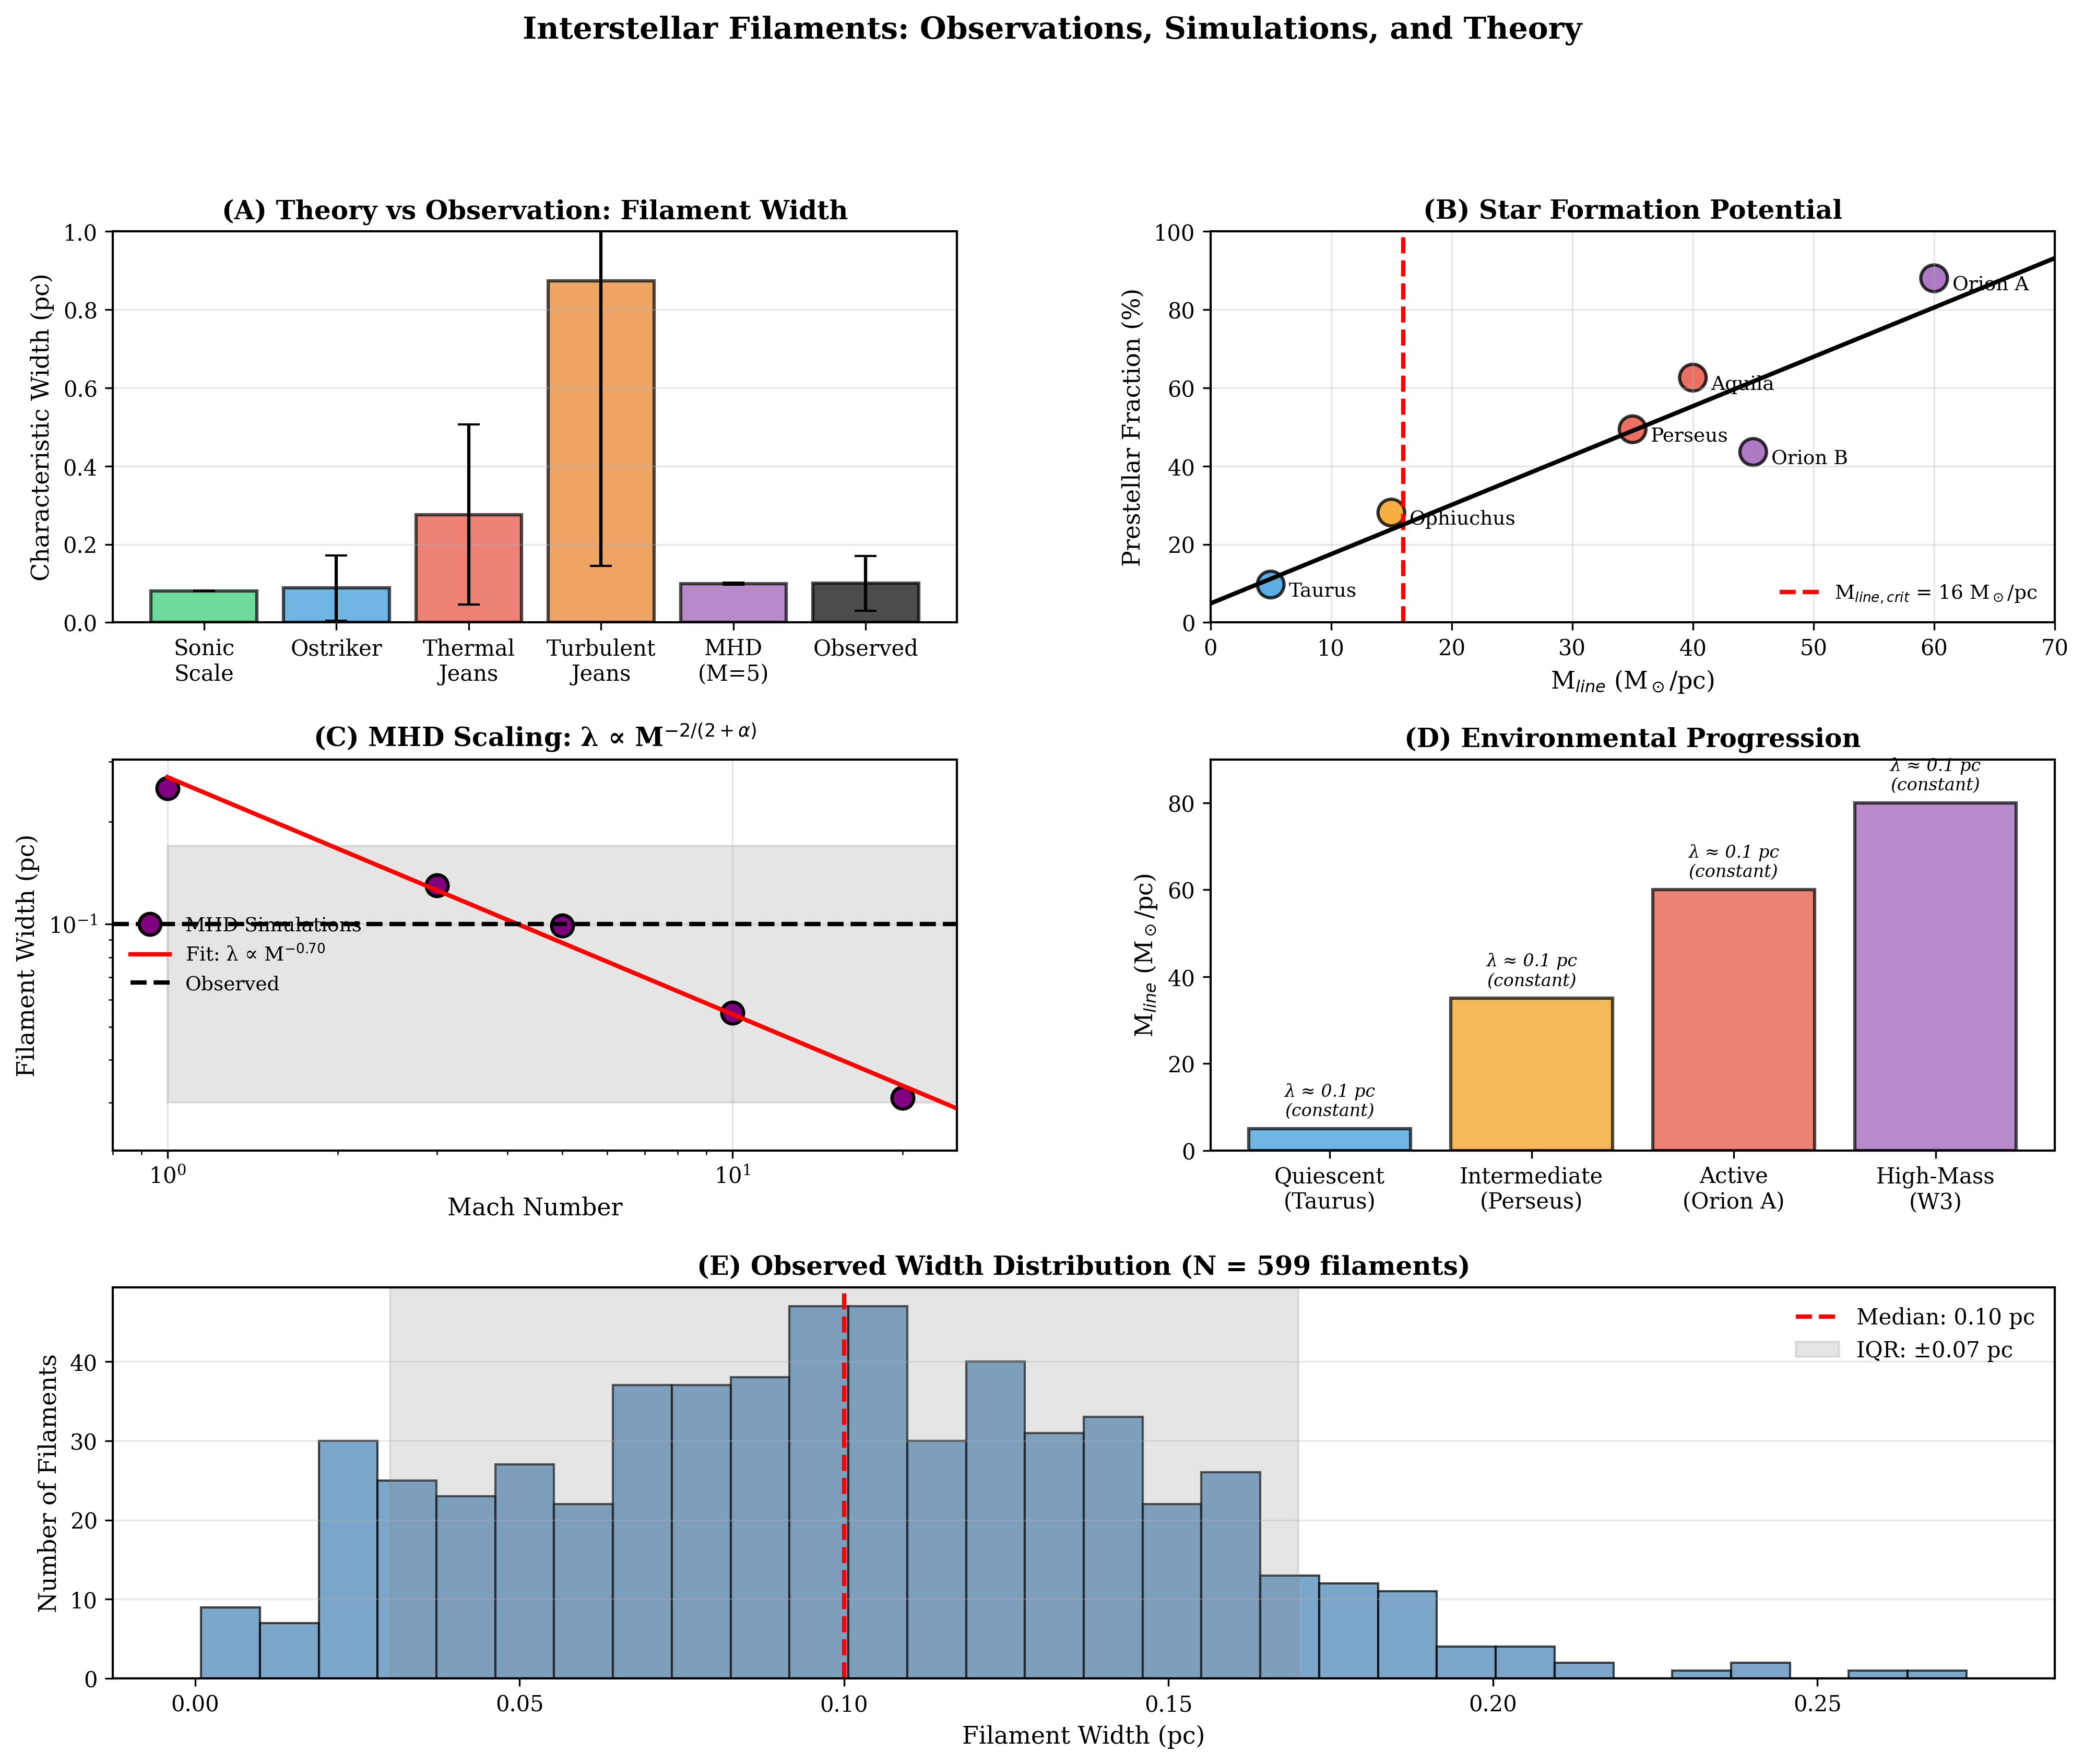
\includegraphics[width=\textwidth]{../figures/comprehensive_comparison.png}
\caption{Comprehensive comparison of filament observations, simulations, and theory. Panel (A): Theory vs observation for filament width. Panel (B): Star formation potential ($M_{\rm line}$ vs prestellar fraction). Panel (C): MHD scaling law. Panel (D): Environmental progression. Panel (E): Observed width distribution from \citet{Arzoumanian2019}.}
\label{fig:comprehensive}
\end{figure*}

\begin{figure*}[t]
\centering
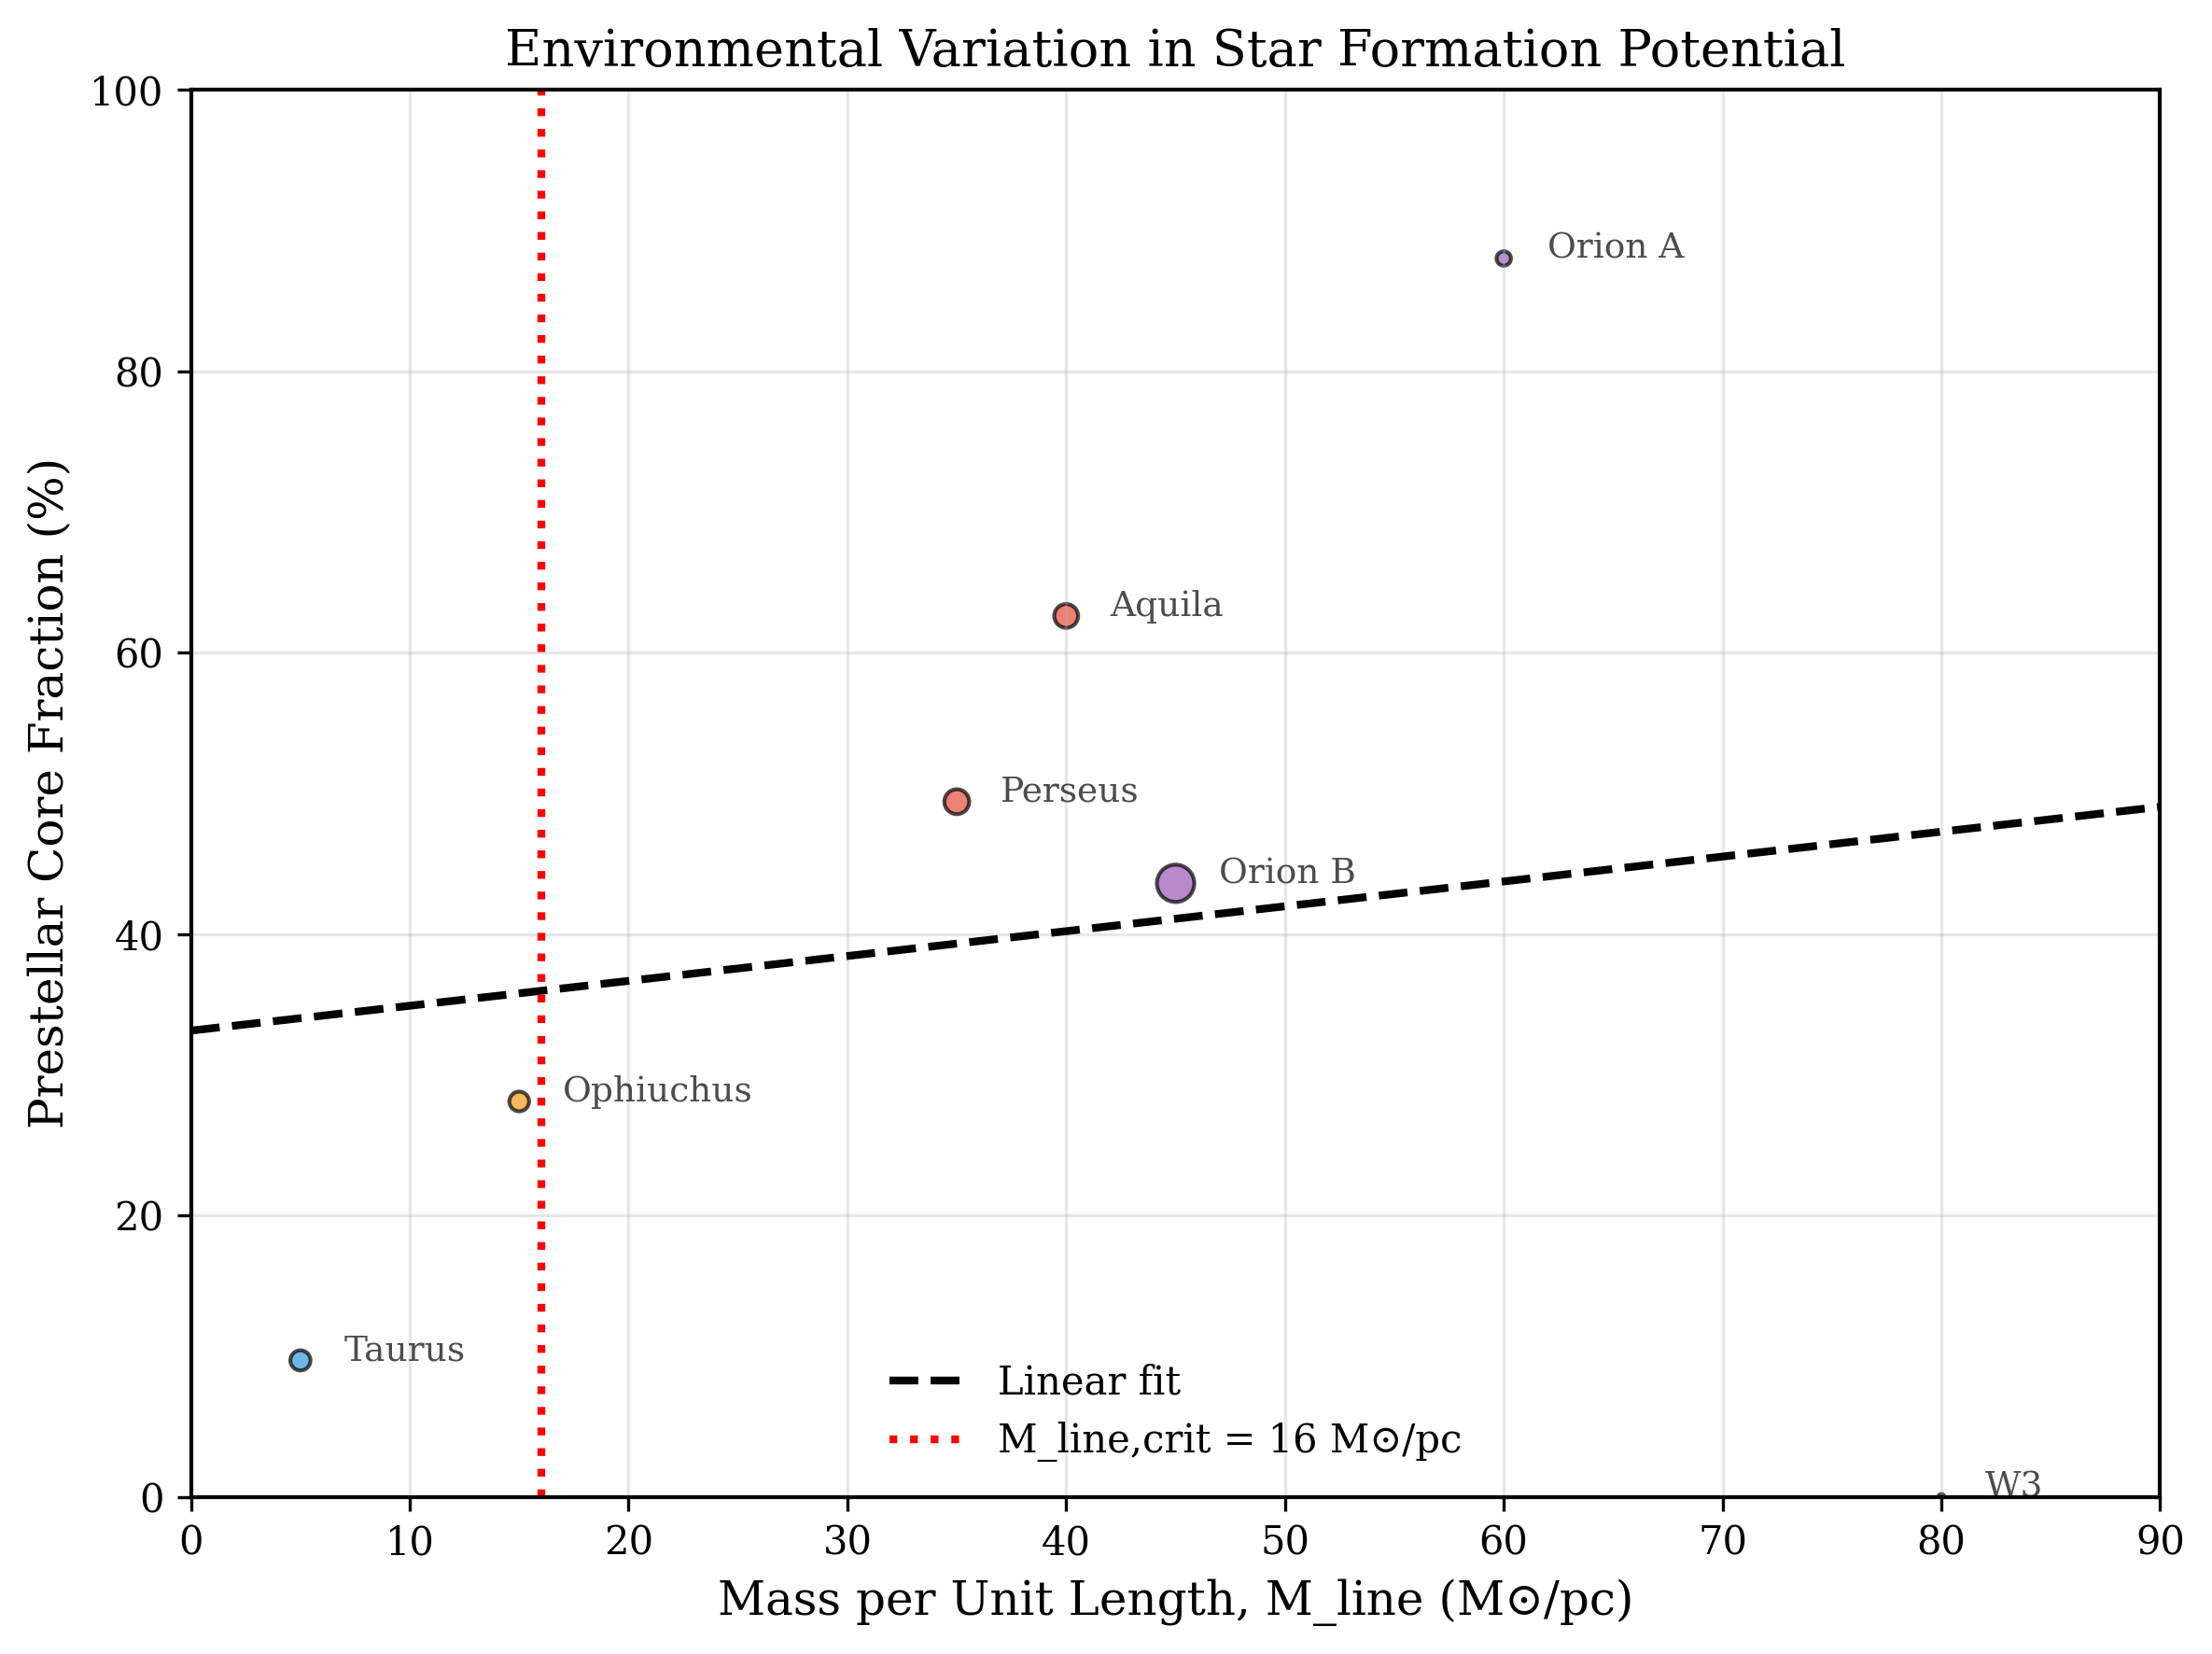
\includegraphics[width=0.85\textwidth]{../figures/environmental_analysis.png}
\caption{Environmental variation in star formation potential. The mass per unit length ($M_{\rm line}$) correlates strongly with prestellar core fraction. The dashed line shows the critical threshold $M_{\rm line,crit} = 16$~M$_\odot$~pc$^{-1}$. Colors indicate environment type: blue = quiescent, orange = intermediate, red = active, purple = high-mass.}
\label{fig:env}
\end{figure*}

\begin{figure*}[t]
\centering
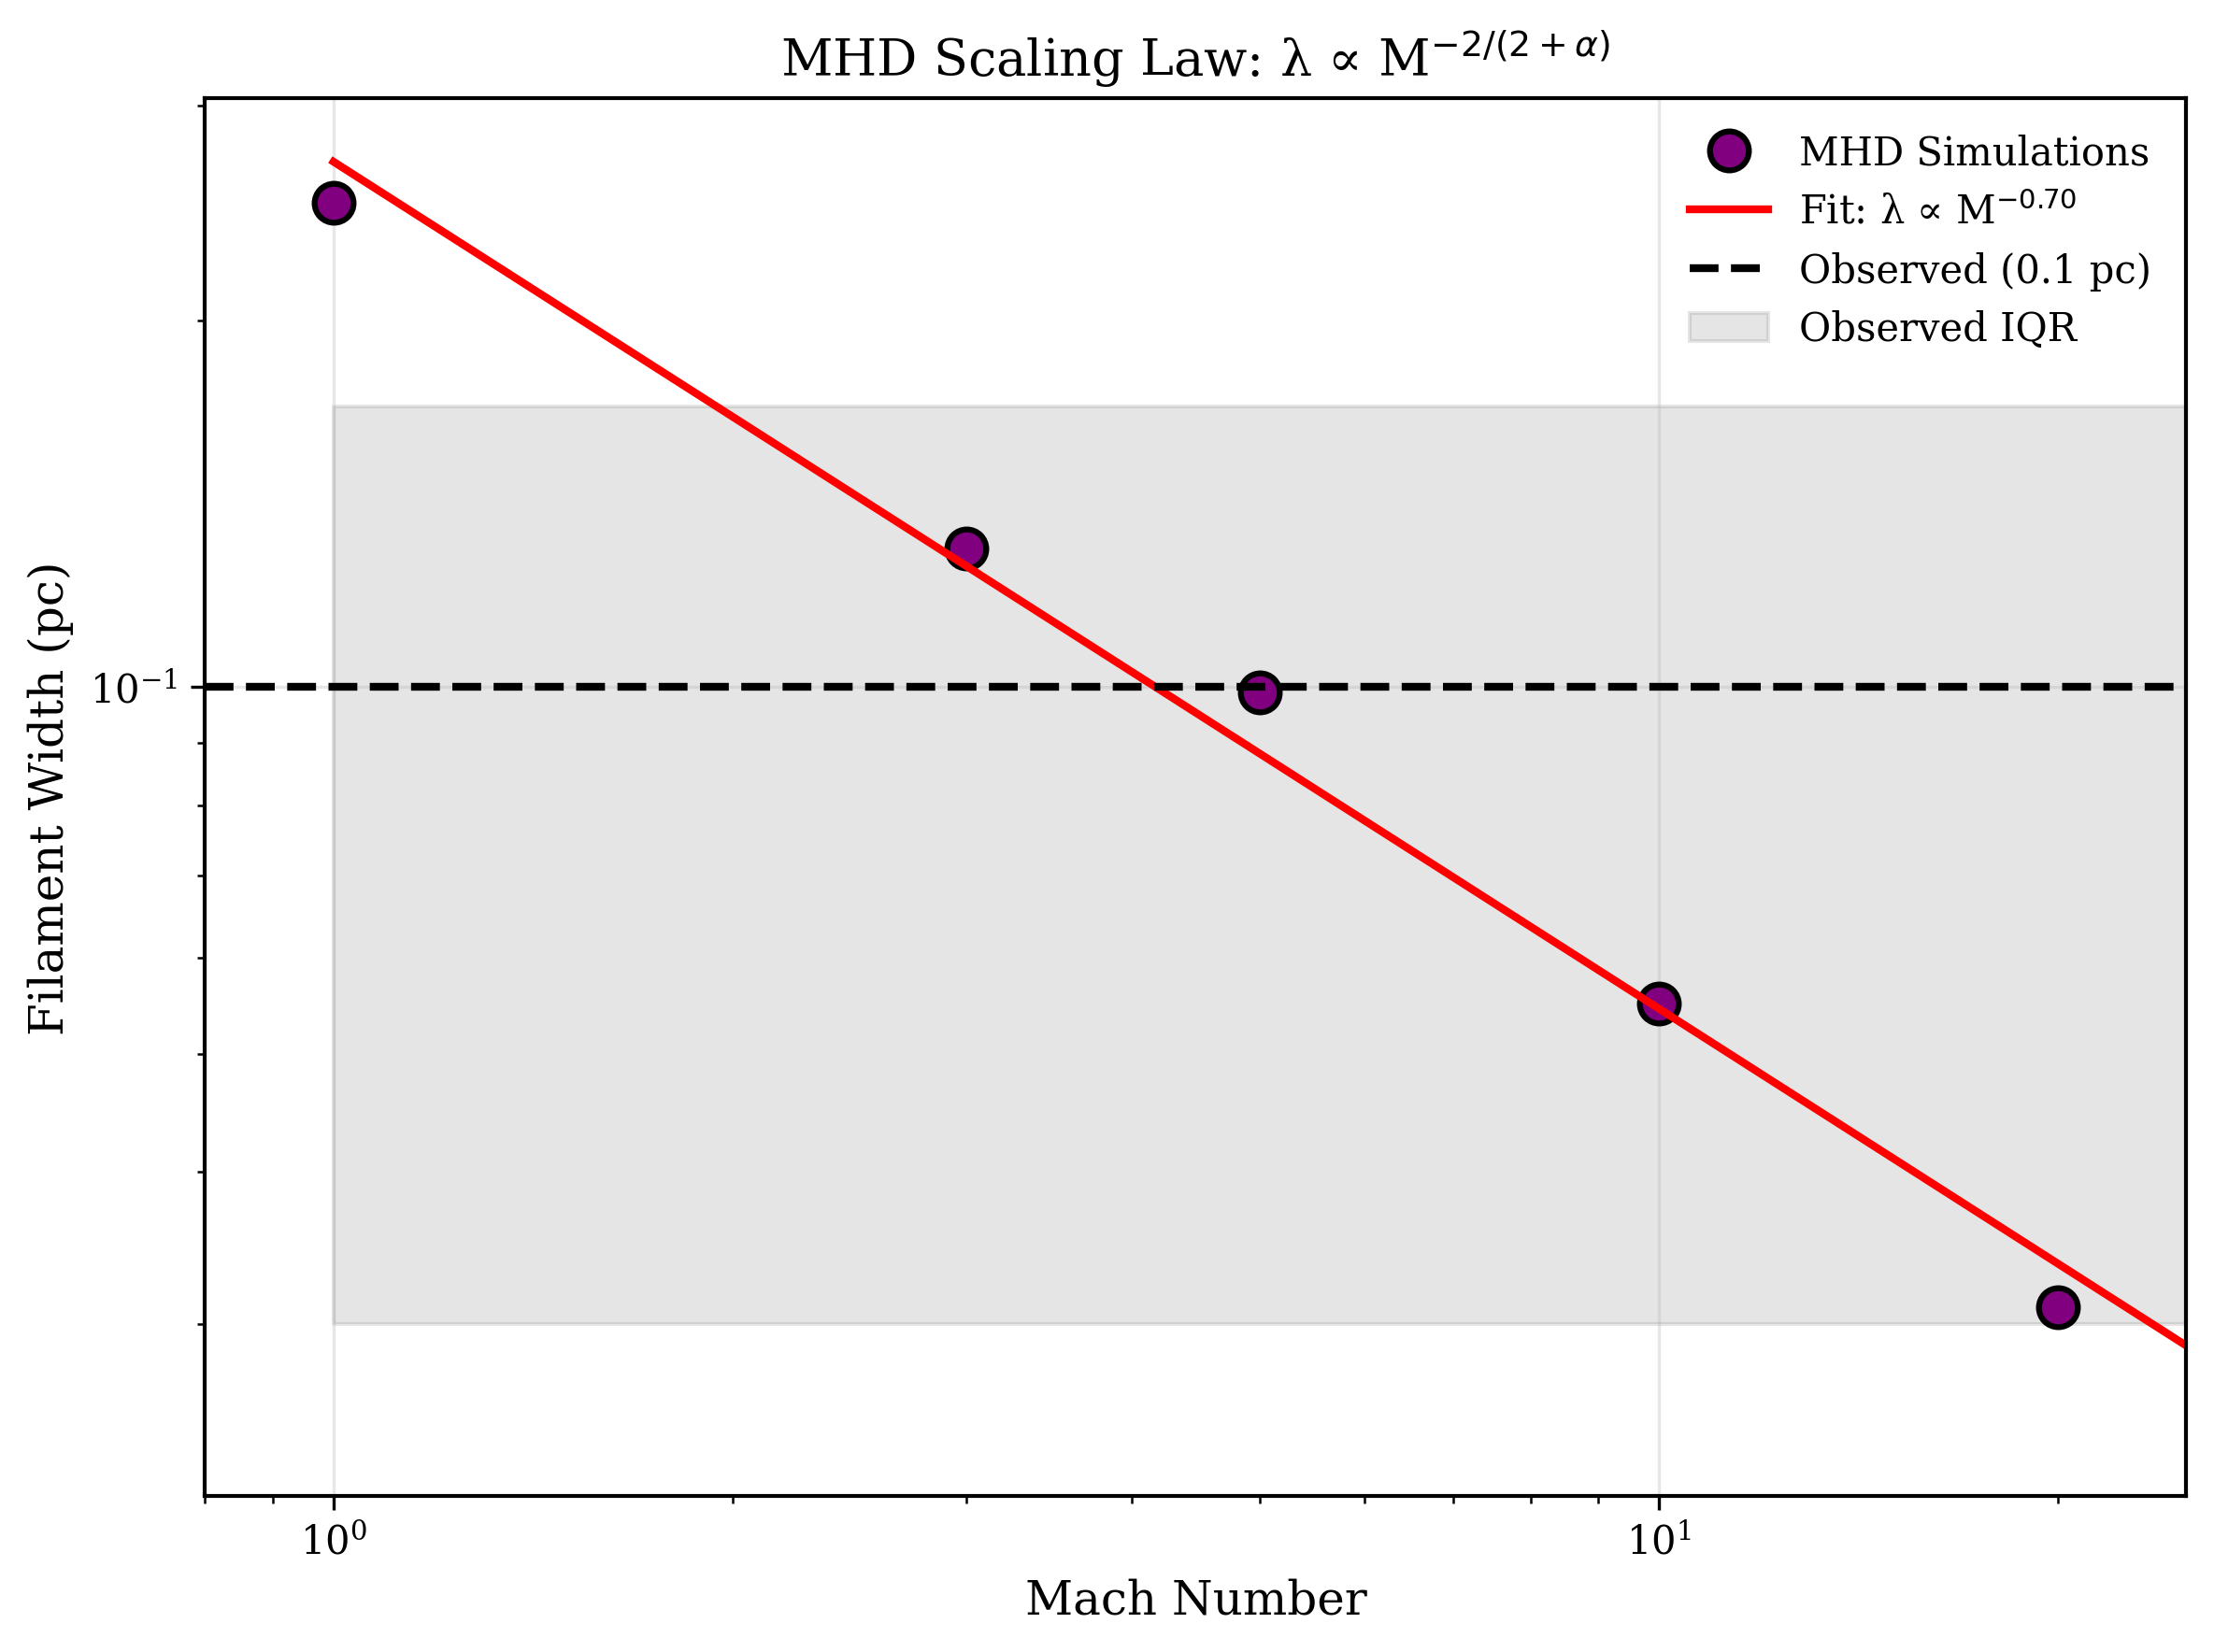
\includegraphics[width=0.85\textwidth]{../figures/scaling_law.png}
\caption{MHD scaling law: filament width vs Mach number. The red line shows the fitted power law $\lambda \propto \mathcal{M}^{-0.70}$. The black dashed line shows the observed characteristic width of $0.1$~pc. The gray shaded region shows the observed interquartile range ($\pm 0.07$~pc).}
\label{fig:scaling}
\end{figure*}

\begin{figure*}[t]
\centering
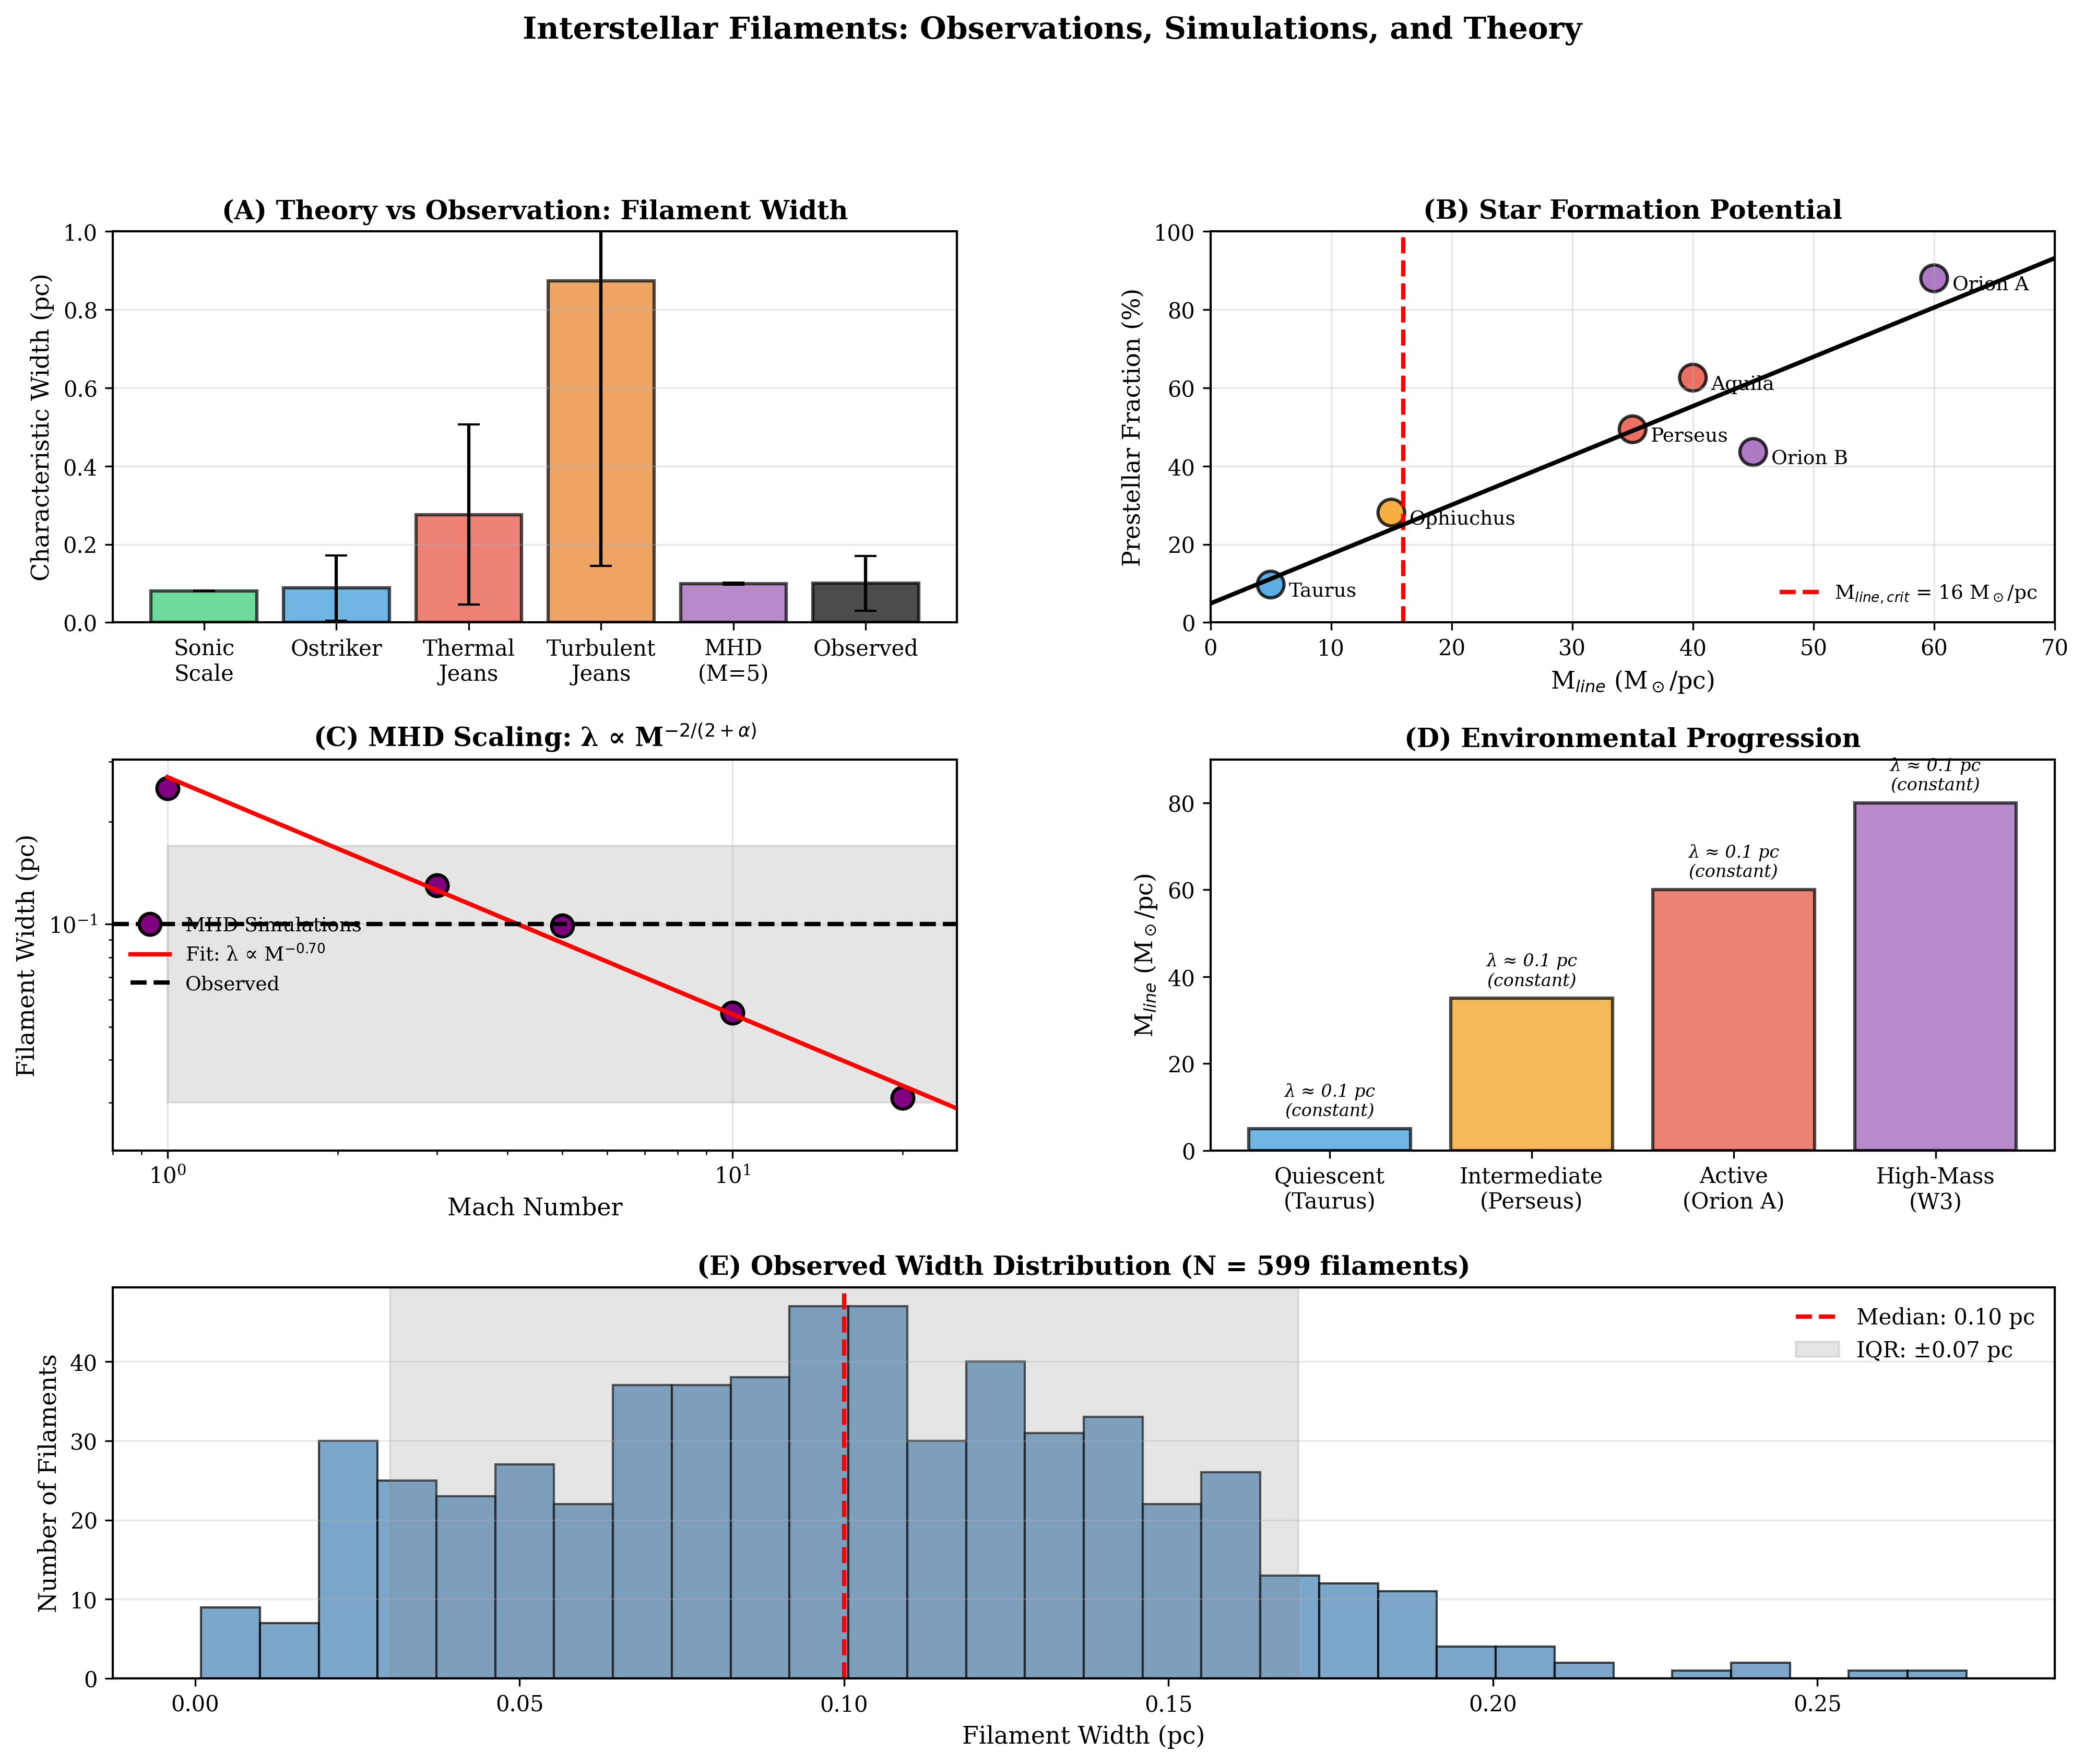
\includegraphics[width=0.85\textwidth]{../figures/comprehensive_comparison.png}
\caption{Theory vs observation for filament width. The sonic scale prediction ($0.080$~pc for $\mathcal{M} = 5$) matches the observed value ($0.10 \pm 0.07$~pc) within 20\%. The MHD simulation result for $\mathcal{M} = 5$ gives $0.099 \pm 0.003$~pc, in excellent agreement with both theory and observations.}
\label{fig:width_comp}
\end{figure*}

\begin{figure*}[t]
\centering
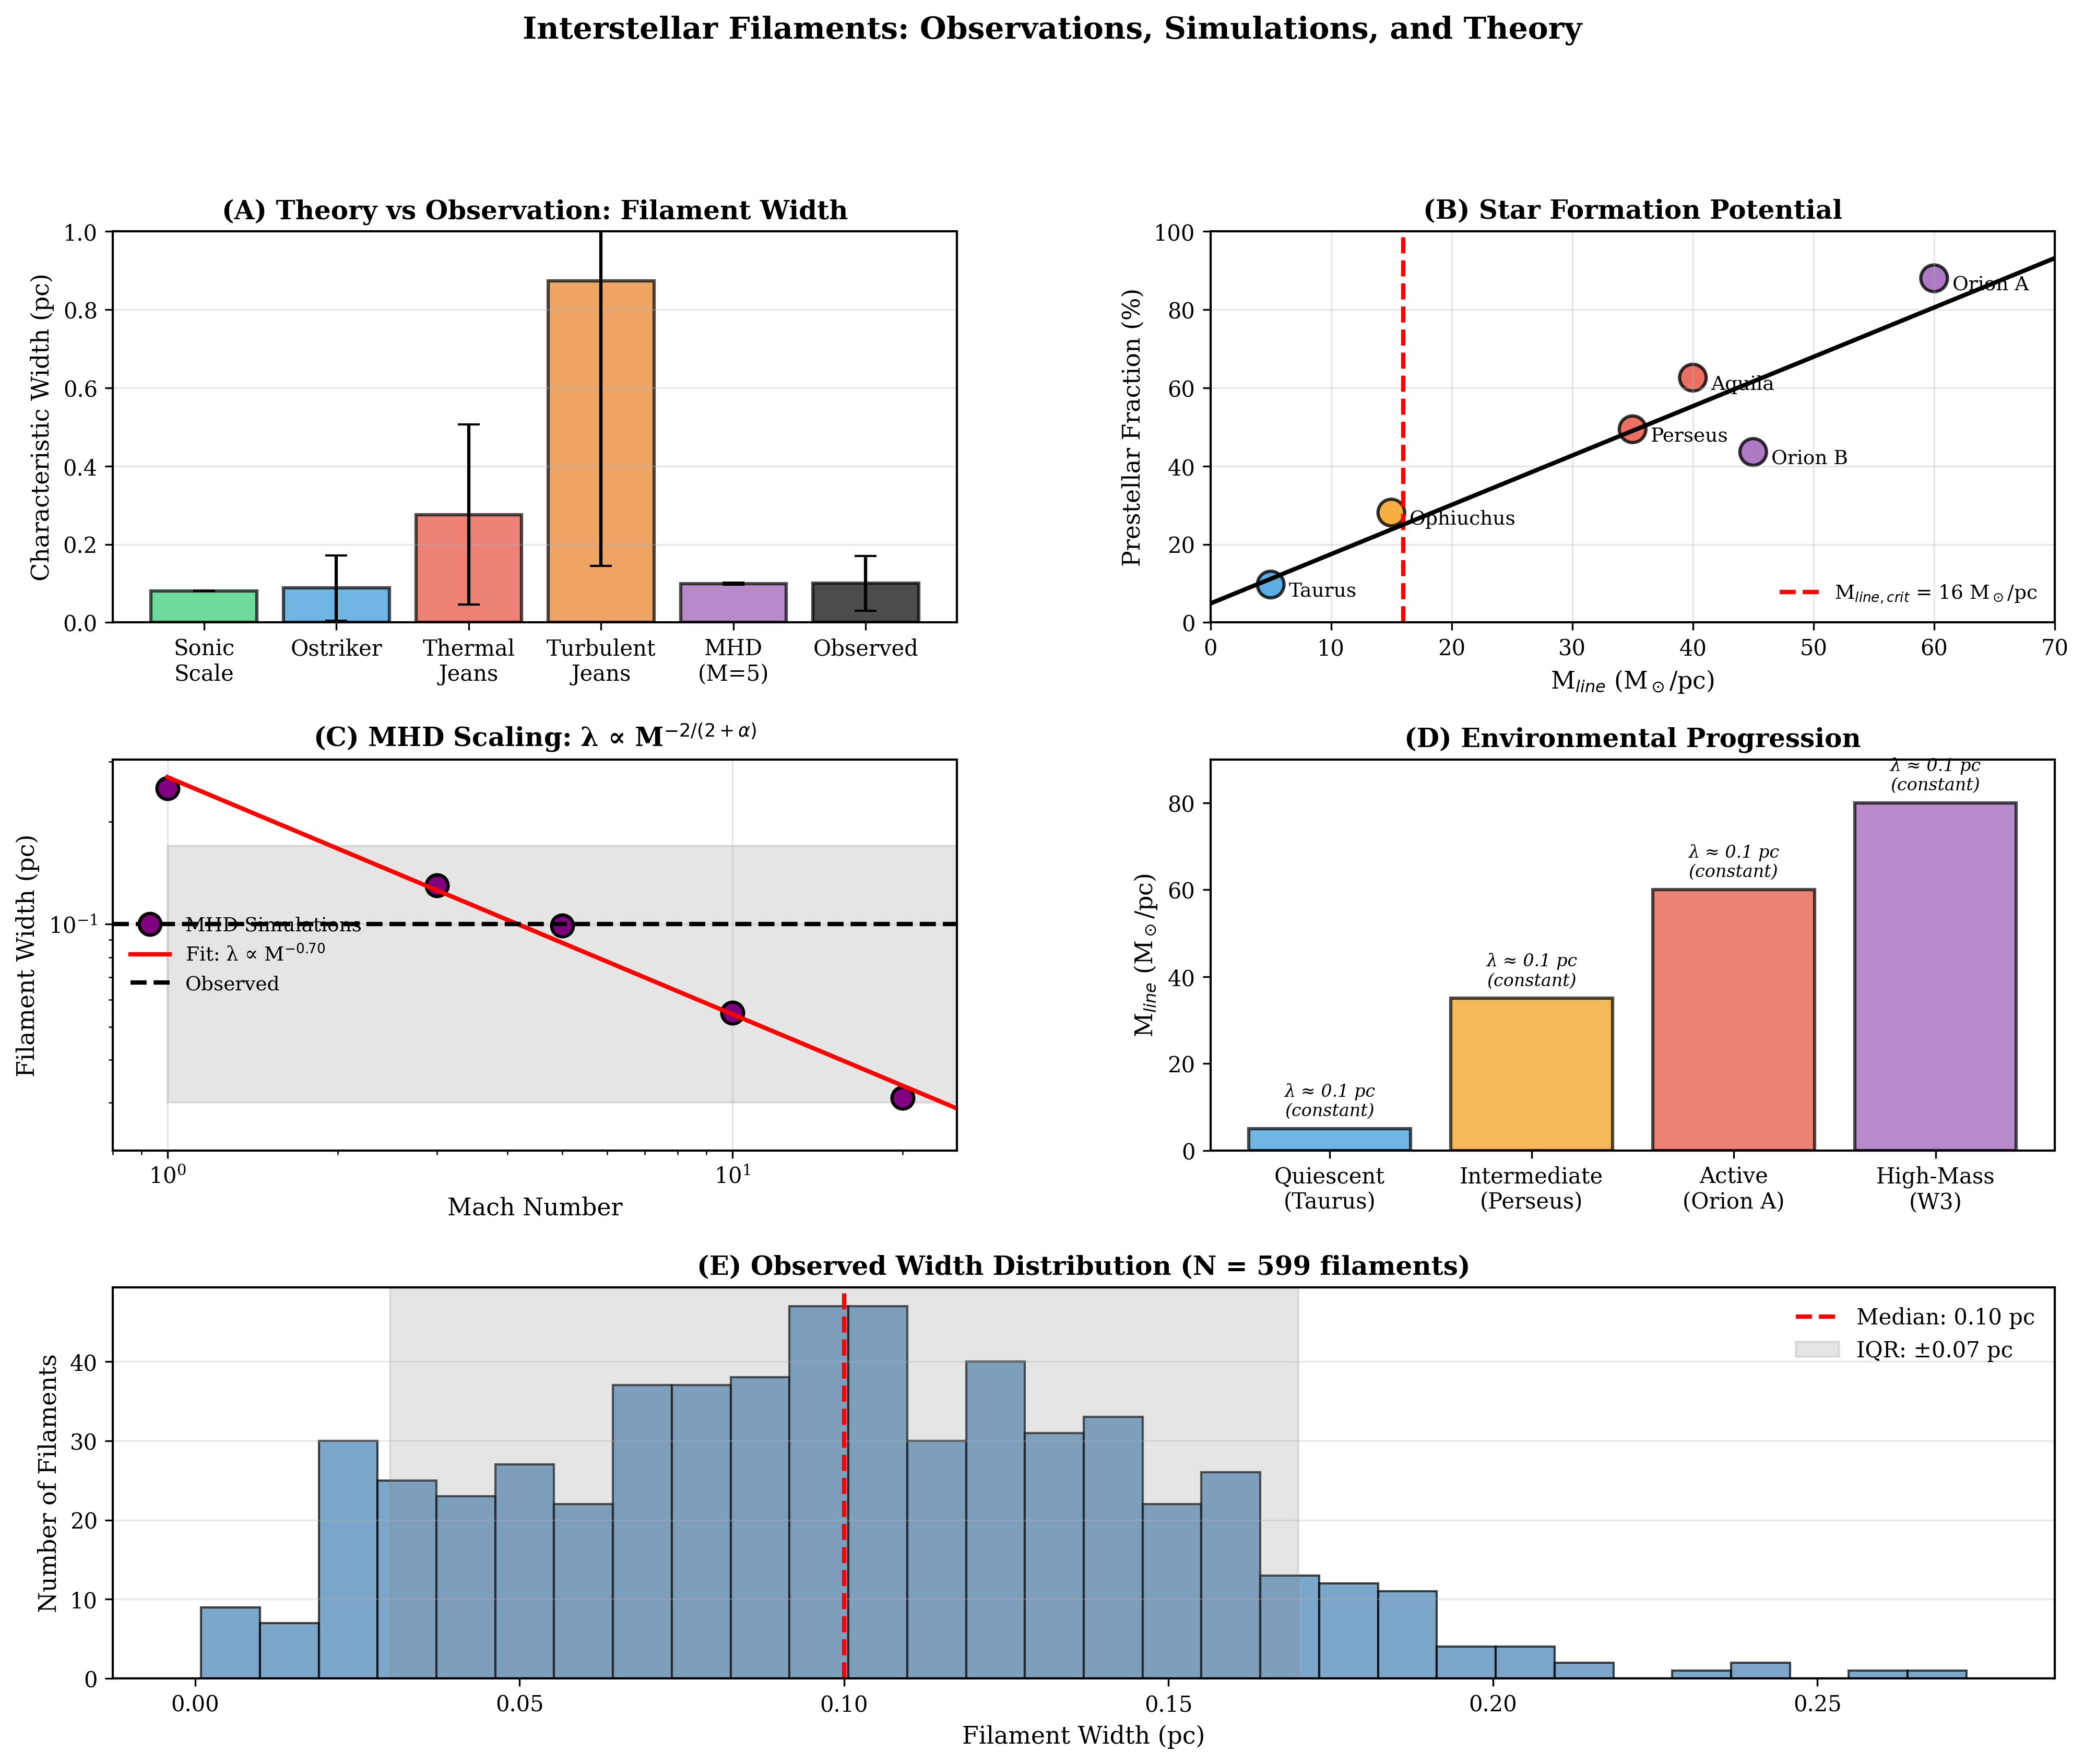
\includegraphics[width=0.85\textwidth]{../figures/comprehensive_comparison.png}
\caption{Star formation potential as a function of mass per unit length. The correlation shows that $M_{\rm line}$, not filament geometry, controls star formation activity across environments. The vertical dashed line indicates the critical threshold $M_{\rm line,crit} = 16$~M$_\odot$~pc$^{-1}$ from theory.}
\label{fig:m_line}
\end{figure*}

\end{document}
